%!TeX root=../tese.tex
%("dica" para o editor de texto: este arquivo é parte de um documento maior)
% para saber mais: https://tex.stackexchange.com/q/78101/183146

%% [p. 3 / § 1] “restrição o escopo” → “restrição do escopo”  : X

% [p. 3 / § 2] Na primeira frase, acho que fica mais claro dizer “grupos com quantidades finitas de inimigos atacam o jogador”, já que é a divisão dos inimigos em grupos de ataque que caracteriza a mecânica de ondas :X

% Figuras 2.1 a 2.3
% citar desenvolvedores :X
% mencionar figuras no texto : X

% Seção 2.3: citar para Spacewar, Space Invaders e Asteroids: X

% [p. 5 / § 2] Adicionar notas de rodapé com URL para sites cada tecnologia, com data do último acesso




%% ------------------------------------------------------------------------- %%
\chapter{Gêneros de Jogos e Decisões de Projeto}
\label{cap:generos-decisoes}

Existe uma infinidade de estilos de jogos que necessitam de oponentes gerados automaticamente contra o jogador, contudo, considerando o algoritmo genético que seria desenvolvido e a restrição do escopo de desenvolvimento do mesmo, decidiu-se por utilizar jogos com ondas de inimigos. Desta forma, o algoritmo poderia considerar a onda como uma população e separar candidatos apropriados para gerar a próxima onda.

%% ------------------------------------------------------------------------- %%
\section{Jogos com Ondas de Inimigos}
\label{sec:jogos-ondas}

Neste estilo de jogo, basicamente, grupos com quantidades finitas de inimigos atacam o jogador, seguindo uma sequência crescente de dificuldade. Em geral as ondas são previamente programadas de acordo com a escala de dificuldade e história que o desenvolvedor deseja demonstrar, mas que podem tornar as partidas repetitivas e facilmente contra-atacadas por jogadores que conseguem abstrair o raciocínio de progresso que foi programado. Ao utilizar um algoritmo genético para produzir as ondas de inimigos, seria possível surpreender o jogador e se adaptar a ele, aumentando a diversidade estratégica e diminuindo a monotonia do jogo.

\pagebreak

%% ------------------------------------------------------------------------- %%
\section{Tower Defense}
\label{sec:jogo-td}

 \textit{Tower defense} é um gênero de jogo onde o jogador deve focar na defesa de território, posicionando defesas limitadas por um recurso - geralmente com a compra de torres que atacam o inimigo - em um caminho pelo qual ondas de oponentes passam, buscando destruir a base do jogador. Pode se citar como exemplo de jogo desse gênero o \textit{game} \textit{Kingdom-rush} \citep{kingdom_rush} que encontra se na Figura \ref{fig:kingdom-rush}. Para impedir que o inimigo percorra o mapa completamente, as torres devem ser posicionadas para maximizar o tempo de ataque e minimizar o custo, levando em consideração que torres e os inimigos podem apresentar habilidades diferentes como maior resistência ou tiros com maior ou menor dano (ou velocidade), cabendo ao jogador determinar como utilizar os recursos disponíveis.
 
Existem jogos que apresentam a possibilidade de melhoria das defesas utilizando recursos acumulados ao eliminar oponentes, assim o jogador pode conseguir alterar e aprimorar a estratégia durante as fases da partida. A seleção e escolha do posicionamento das torres é a estratégia essencial do jogo.

%% https://www.ironhidegames.com/Games/kingdom-rush
\begin{figure}
  \centering
  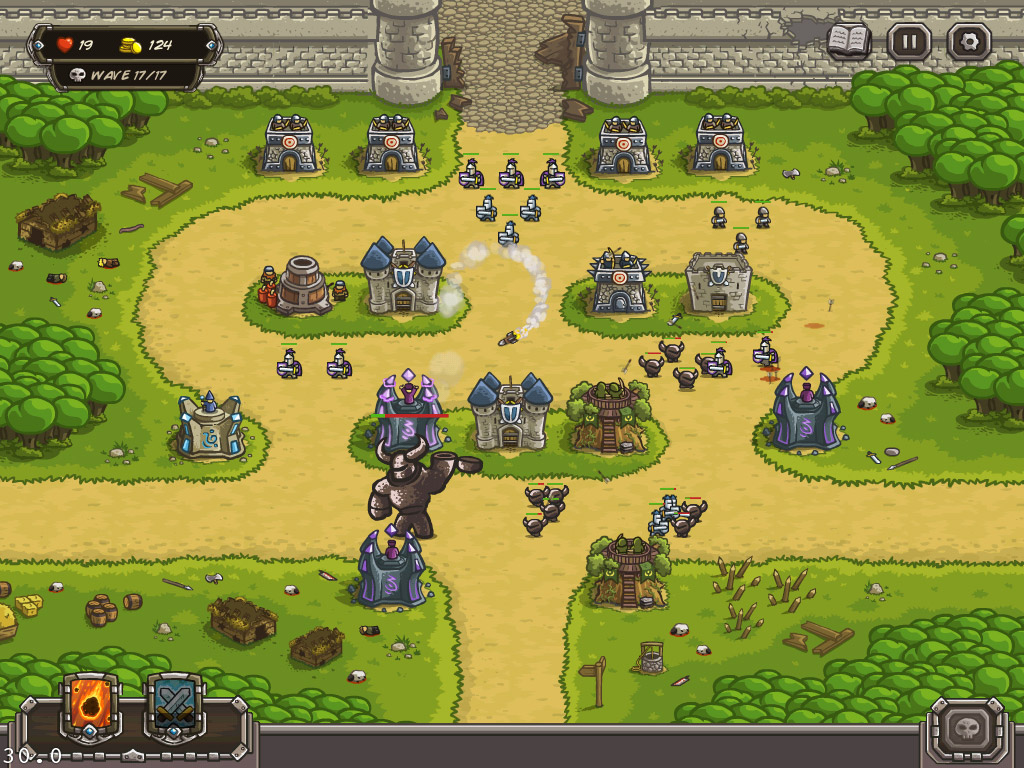
\includegraphics[width=.8\textwidth]{kingdom_rush}
  \caption{Kingdom Rush. Obtida de https://www.ironhidegames.com/Games/kingdom-rush\label{fig:kingdom-rush}}
\end{figure}

\pagebreak

%% ------------------------------------------------------------------------- %%
\section{Shooter}
\label{sec:jogo-ss}

Um \textit{shooter game} é um subgênero de jogos de ação, inspirado pelos jogos de fliperama, por exemplo o jogo  \textit{Spacewar} \citep{Spacewar}, e se estabeleceu com o jogo \textit{Space Invaders} \citep{Space_Invaders}, presente na Figura \ref{fig:space-invaders}. Ambos os jogos funcionam de maneira semelhante, onde uma onda de inimigos deve ser impedida de eliminar o jogador, este podendo se esquivar e atirar neles, sendo que os oponentes também podem dispor de tiros e movimento para causar dano.

%% https://www.gamekult.com/jeux/space-invaders-17318/test.html
\begin{figure}
  \centering
  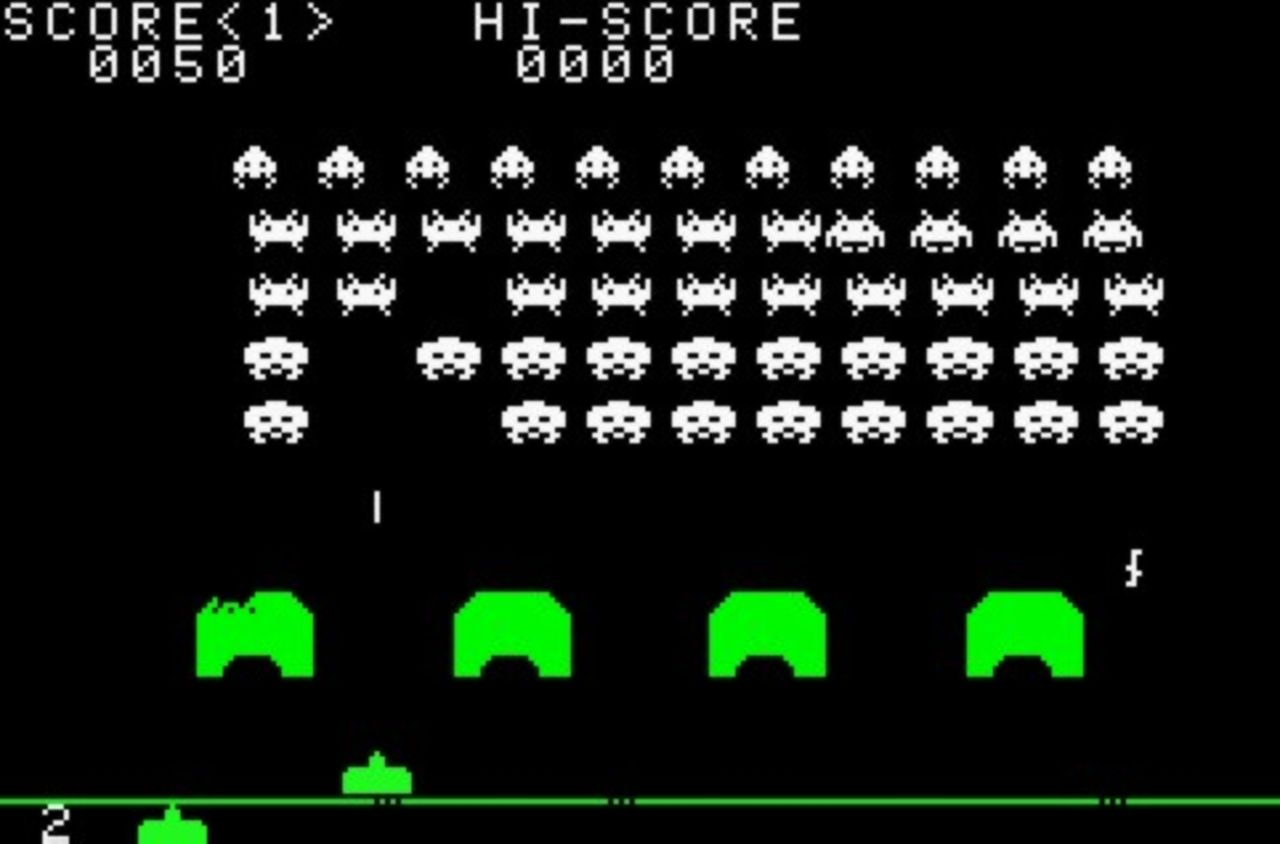
\includegraphics[width=.6\textwidth]{space_invaders}
  \caption{Space Invaders. Obtida de https://www.gamekult.com/jeux/space-invaders-17318/test.html\label{fig:space-invaders}}
\end{figure}

Dentre os elementos comuns ao gênero, existem variações sobre a capacidade do jogador e dos inimigos se moverem no espaço 2D, onde no \textit{Space Invaders} \citep{Space_Invaders}, o jogador possui somente movimento horizontal, enquanto no \textit{Asteroids} \citep{Asteroids}, presente na Figura \ref{fig:asteroids}, o usuário possui movimentação livre em toda área disponível, mas os oponentes não disparam.

%% https://openclipart.org/detail/281726/asteroids-video-games-1979
\begin{figure}
  \centering
  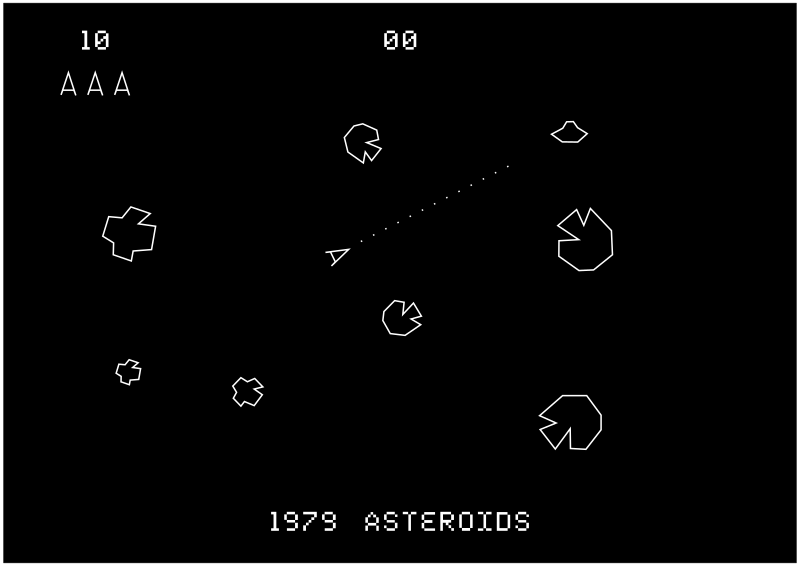
\includegraphics[width=.6\textwidth]{asteroids}
  \caption{Asteroids. Obtida de https://openclipart.org/detail/281726/asteroids-video-games-1979\label{fig:asteroids}}
\end{figure}

%% ------------------------------------------------------------------------- %%
\section{Decisões de Projeto}
\label{sec:jogos-decisoes}

Considerando que são jogos populares e com jogabilidade simples, decidiu-se desenvolver os dois estilos, considerando a simplicidade de seus objetivos em comum, centrados na sobrevivência por meio da habilidade do jogador de se proteger dos inimigos que atacam em turnos, e a possibilidade dos mesmos serem eliminados à distância.

Ao mesmo tempo, enquanto o \textit{Tower Defense} se apresenta de maneira estática - as torres não se movem, e o jogador não pode alterá-las durante a onda - o \textit{Space Shooter} permite movimentação da nave, logo a habilidade motora e reflexos de quem está jogando são fatores na sobrevivência, e seria interessante verificar como essa característica afeta a evolução do algoritmo genético.

Para desenvolver o projeto decidiu-se utilizar ferramentas \textit{Open Source} sempre que possível, a \textit{Godot Game Engine}, versão 3.3.3; a plataforma de versionamento \textit{GitHub}; a comunicação do grupo se concentrou no serviço \textit{Discord}; a monografia foi desenvolvida de maneira colaborativa na plataforma \textit{OverLeaf}; o \textit{Jupyter Notebook} foi utilizado para análise de dados; e o editor de imagens \textit{GIMP} para edição de imagens.